%%%%%%%%%%%%%%%%%%%%%%%%%%%%%%%%%%%%%%%%%
% Article EcoFoG
% Version 2.1 (23/10/2017)
%
% adapté de :
% Stylish Article
% LaTeX Template
% Version 1.0 (31/1/13)
%
% This template has been downloaded from:
% http://www.LaTeXTemplates.com
%
% Original author:
% Mathias Legrand (legrand.mathias@gmail.com)
%
% License:
% CC BY-NC-SA 3.0 (http://creativecommons.org/licenses/by-nc-sa/3.0/)
%
%%%%%%%%%%%%%%%%%%%%%%%%%%%%%%%%%%%%%%%%%


%----------------------------------------------------------------------------------------
%	PACKAGES AND OTHER DOCUMENT CONFIGURATIONS
%----------------------------------------------------------------------------------------

\documentclass[fleqn,10pt]{ArtEcoFoG} % Document font size and equations flushed left

\setcounter{tocdepth}{3} % Show only three levels in the table of contents section: sections, subsections and subsubsections


% Pandoc environments
\usepackage{framed}
\usepackage{fancyvrb}
\providecommand{\tightlist}{%
  \setlength{\itemsep}{0pt}\setlength{\parskip}{0pt}}
\newcommand{\VerbBar}{|}
\newcommand{\VERB}{\Verb[commandchars=\\\{\}]}
\DefineVerbatimEnvironment{Highlighting}{Verbatim}{commandchars=\\\{\}, fontsize=\scriptsize} % Code R
\definecolor{shadecolor}{RGB}{248,248,248}
\newenvironment{Shaded}{\begin{snugshade}}{\end{snugshade}}
\newcommand{\KeywordTok}[1]{\textcolor[rgb]{0.13,0.29,0.53}{\textbf{{#1}}}}
\newcommand{\DataTypeTok}[1]{\textcolor[rgb]{0.13,0.29,0.53}{{#1}}}
\newcommand{\DecValTok}[1]{\textcolor[rgb]{0.00,0.00,0.81}{{#1}}}
\newcommand{\BaseNTok}[1]{\textcolor[rgb]{0.00,0.00,0.81}{{#1}}}
\newcommand{\FloatTok}[1]{\textcolor[rgb]{0.00,0.00,0.81}{{#1}}}
\newcommand{\ConstantTok}[1]{\textcolor[rgb]{0.00,0.00,0.00}{{#1}}}
\newcommand{\CharTok}[1]{\textcolor[rgb]{0.31,0.60,0.02}{{#1}}}
\newcommand{\SpecialCharTok}[1]{\textcolor[rgb]{0.00,0.00,0.00}{{#1}}}
\newcommand{\StringTok}[1]{\textcolor[rgb]{0.31,0.60,0.02}{{#1}}}
\newcommand{\VerbatimStringTok}[1]{\textcolor[rgb]{0.31,0.60,0.02}{{#1}}}
\newcommand{\SpecialStringTok}[1]{\textcolor[rgb]{0.31,0.60,0.02}{{#1}}}
\newcommand{\ImportTok}[1]{{#1}}
\newcommand{\CommentTok}[1]{\textcolor[rgb]{0.56,0.35,0.01}{\textit{{#1}}}}
\newcommand{\DocumentationTok}[1]{\textcolor[rgb]{0.56,0.35,0.01}{\textbf{\textit{{#1}}}}}
\newcommand{\AnnotationTok}[1]{\textcolor[rgb]{0.56,0.35,0.01}{\textbf{\textit{{#1}}}}}
\newcommand{\CommentVarTok}[1]{\textcolor[rgb]{0.56,0.35,0.01}{\textbf{\textit{{#1}}}}}
\newcommand{\OtherTok}[1]{\textcolor[rgb]{0.56,0.35,0.01}{{#1}}}
\newcommand{\FunctionTok}[1]{\textcolor[rgb]{0.00,0.00,0.00}{{#1}}}
\newcommand{\VariableTok}[1]{\textcolor[rgb]{0.00,0.00,0.00}{{#1}}}
\newcommand{\ControlFlowTok}[1]{\textcolor[rgb]{0.13,0.29,0.53}{\textbf{{#1}}}}
\newcommand{\OperatorTok}[1]{\textcolor[rgb]{0.81,0.36,0.00}{\textbf{{#1}}}}
\newcommand{\BuiltInTok}[1]{{#1}}
\newcommand{\ExtensionTok}[1]{{#1}}
\newcommand{\PreprocessorTok}[1]{\textcolor[rgb]{0.56,0.35,0.01}{\textit{{#1}}}}
\newcommand{\AttributeTok}[1]{\textcolor[rgb]{0.77,0.63,0.00}{{#1}}}
\newcommand{\RegionMarkerTok}[1]{{#1}}
\newcommand{\InformationTok}[1]{\textcolor[rgb]{0.56,0.35,0.01}{\textbf{\textit{{#1}}}}}
\newcommand{\WarningTok}[1]{\textcolor[rgb]{0.56,0.35,0.01}{\textbf{\textit{{#1}}}}}
\newcommand{\AlertTok}[1]{\textcolor[rgb]{0.94,0.16,0.16}{{#1}}}
\newcommand{\ErrorTok}[1]{\textcolor[rgb]{0.64,0.00,0.00}{\textbf{{#1}}}}
\newcommand{\NormalTok}[1]{{#1}}
\usepackage{longtable,booktabs}
\usepackage{caption}
% These lines are needed to make table captions work with longtable:
\makeatletter
\def\fnum@table{\tablename~\thetable}
\makeatother
% longtable 2 columns
% https://tex.stackexchange.com/questions/161431/how-to-solve-longtable-is-not-in-1-column-mode-error
\makeatletter
\let\oldlt\longtable
\let\endoldlt\endlongtable
\def\longtable{\@ifnextchar[\longtable@i \longtable@ii}
\def\longtable@i[#1]{\begin{figure}[t]
\onecolumn
\begin{minipage}{0.5\textwidth}\scriptsize
\oldlt[#1]
}
\def\longtable@ii{\begin{figure}[t]
\onecolumn
\begin{minipage}{0.5\textwidth}\scriptsize
\oldlt
}
\def\endlongtable{\endoldlt
\end{minipage}
\twocolumn
\end{figure}}
\makeatother

\usepackage{graphicx,grffile}
\makeatletter
\def\maxwidth{\ifdim\Gin@nat@width>\linewidth\linewidth\else\Gin@nat@width\fi}
\def\maxheight{\ifdim\Gin@nat@height>\textheight0.8\textheight\else\Gin@nat@height\fi}
\makeatother
% Scale images if necessary, so that they will not overflow the page
% margins by default, and it is still possible to overwrite the defaults
% using explicit options in \includegraphics[width, height, ...]{}
\setkeys{Gin}{width=\maxwidth,height=\maxheight,keepaspectratio}

% User-adder preamble
\usepackage{textcomp} \DeclareUnicodeCharacter{B0}{\textdegree}
\usepackage{tabu}
\renewenvironment{table}{\begin{table*}}{\end{table*}\ignorespacesafterend}
\hyphenation{bio-di-ver-si-ty sap-lings}

%----------------------------------------------------------------------------------------
%	ARTICLE INFORMATION
%----------------------------------------------------------------------------------------

\JournalInfo{Hal 00679993} % Journal information
\Archive{DOI xxxx} % Additional notes (e.g. copyright, DOI, review/research article)

\PaperTitle{30 Years of Recruitment in Tropical Forest After Selective Logging} % Article title

\Authors{
Ariane MIRABEL\textsuperscript{1*}\\ Eric MARCON\textsuperscript{1}\\ Bruno HERAULT\textsuperscript{2}
} % Authors
\affiliation{
\textsuperscript{1}UMR EcoFoG, AgroParistech, CNRS, Cirad, INRA, Université des Antilles,
Université de Guyane.\\ \hspace{1em} Campus Agronomique, 97310 Kourou, France.\\\textsuperscript{2}INPHB (Institut National Ploytechnique Félix Houphoüet Boigny)\\ \hspace{1em} Yamoussoukro, Ivory Coast
}
\affiliation{*\textbf{Contact}: ariane.mirabel@ecofog.gf, http://www.ecofog.gf/spip.php?article47} % Corresponding author

\Keywords{mot-clés, séparés par des virgules} % Keywords - if you don't want any simply remove all the text between the curly brackets
\newcommand{\keywordname}{Mots-clés} % Defines the keywords heading name

%----------------------------------------------------------------------------------------
%	ABSTRACT
%----------------------------------------------------------------------------------------

\Abstract{
Résumé de l'article.
}

%----------------------------------------------------------------------------------------

\begin{document}

\selectlanguage{english}

\flushbottom % Makes all text pages the same height

\maketitle % Print the title and abstract box

\tableofcontents % Print the contents section

\thispagestyle{empty} % Removes page numbering from the first page

%----------------------------------------------------------------------------------------
%	ARTICLE CONTENTS
%----------------------------------------------------------------------------------------


\begin{verbatim}
## Warning: package 'kableExtra' was built under R version 3.3.3
\end{verbatim}

\section{Introduction}\label{introduction}

Determining the response of tropical forests to disturbance is a key to
predict their fate in a global change context. A vast literature has
successfully modeled the response of tropical forest dynamics, carbon
stocks and fluxes to anthropogenic and natural disturbances
\citep{Gourlet-Fleury2000, Putz2012, Martin2015, Piponiot2016}. However,
regarding diversity, similar attempts have been hindered by both the
huge biological diversity and the scarcity of long-term monitoring.
Although the community composition response to disturbance was
identified for common species assemblages, this approach is usually
confined to few commercial and valuable species
\citep{Sebbenn2008, Rozendaal2010, Vinson2015}. Given the complexity of
adressing simultaneously the response of dozens of species,
community-scale approaches have been developped \citep{DeAvila2016}.

The post-disturbance community dynamic is largely determined by the
recruitment process, i.e.~from seed production, dispersion and
germination to seedlings' and saplings' growth until a threshold,
usually 10cm DBH in tropical forest plots. Major ecological processes,
such as environmental filtering or limiting similarity, occur before
formal recruitment and determine the taxonomic composition of trees
eventually integrating the forest community \citep{Ackerly2003}. The
recruitment process is inherently linked to the disturbance regime that
locally changes ecosystem's biotic and abiotic conditions and creates
opportunities for pioneer species to strive in the long term rather than
undergoing the competitive exclusion for resources in mature patches
\citep{Denslow1980}. This relies on the Intermediate Disturbance
Hypothesis (IDH) that explains the maintenance of tropical forests
biodiversity by the patchy variability of environmental conditions in
space and time \citep{Guitet2018}. This disturbance-induced
environmental variability, when not too intense, is assumed to enlarge
the ecological range of species present in the community
\citep{Molino2001, Bongers2009} and shapes its taxonomic diversity,
vegetative structure, physiology as well as carbon, nutrients, and water
cycles \citep{Anderson-Teixeira2013}. Empirical tests of the IDH in
tropical rainforests, though, proved hard to succeed and yielded
controversial results \citep{Hubbell1999, Molino2001, Sheil2003}.

During post-disturbance times, the shift from resource-acquisitive to
resource-conservative ecological strategies may be detected in leaves
(leaf thickness, toughness, chlorophyll content and specific area) and
stem (wood specific gravity and bark thickness) and life-history traits
(maximum height at adult stage and class of seed mass)
\citep{Wright2004, Chave2009b, Herault2011}. The relative importance of
recruitment of new individuals and of mortality of distrubance survivors
will shape the new forest and its functioning. Given that disturbance
survivors largely mirror the pre-disturbance forest composition
\citep{Piponiot2018}, predicting the recruitment composition and
diversity trajectories would be a major step towards the prediction of
the future of tropical forest in a changing global environment where
disturbance are expected to become more and more frequent. This would
give insights into the resilience of this hyperdiverse ecosystems,
elucidate the determinism, or not, of tropical forests trajectories,
test the convergence after disturbance of taxonomic and functional
communities towards initial state and also help future adaptative
conservation strategies \citep{Diaz2005, Gardner2007, Schwartz2017}.

In this paper we follow the fate of a recruited tree communities (60121
individuals) over 30 years on a disturbance gradient, with 10 to 60\% of
forest biomass removed. We assessed the taxonomic as well as functional
diversity of recruited trees, using a large functional trait database
covering, the leaf, wood and life-history spectra. We aimed to (i)
assess the role of environmental filtering selecting the recruited trees
according to their competitivity for resource acquisition, (ii) resolve
the convergence of communities and the maintenance of taxonomic
composition in the long term, and (iii) determine the global resilience
of the ecosystem.

\section{Material and Methods}\label{material-and-methods}

\subsection{Study Site}\label{study-site}

The Paracou station is located in a lowland tropical rain forest in
French Guiana (5°18'N and 52°53'W). Climate is tropical wet with mean
annual precipitation averaging 2980 mm.y\textsuperscript{-1} (30-y
period) and a 3-months dry season (\textless{} 100
mm.months\textsuperscript{-1}) from mid-August to mid-November, and a
one-month dry season in March \citep{Wagner2011}. Elevation ranges from
5 to 50 m and mean annual temperature is 26°C. Soils are thin acrisols
over a layer of transformed saprolite with low permeability generating
lateral drainage during heavy rains. The disturbance experiment spread
over a network of twelve 6.25ha plots (Table \ref{tab:Tab1}) that
underwent three disturbance treatments in 1986-1987 \citep{Herault2018}.
Dominant families are Fabaceae, Chrysobalanaceae, Lecythidaceae and
Sapotaceae.

\begin{table}

\caption{\label{tab:Tab1}Intervention table, summary of the disturbance intensity for the 4 plot treatments in Paracou.}
\centering
\begin{tabu} to \linewidth {>{\raggedright}X>{\raggedright}X>{\raggedright}X>{\raggedright}X>{\raggedright}X}
\toprule
Treatment & Timber & Thinning & Fuelwood & \%AGB lost\\
\midrule
Control &  &  &  & 0\\
T1 & DBH $\geq$ 50 cm, commercial species, $\approx$ 10 trees/ha &  &  & $[12\%-33\%]$\\
T2 & DBH $\geq$ 50 cm, commercial species, $\approx$ 10 trees/ha & DBH $\geq$ 40 cm, non-valuable species, $\approx$ 30 trees/ha &  & $[33\%-56\%]$\\
T3 & DBH $\geq$ 50 cm, commercial species, $\approx$ 10 trees/ha & DBH $\geq$ 50 cm, non-valuable species, $\approx$ 15 trees/ha & 40 cm $\leq$ DBH $\leq$ 50 cm, non-valuable species, $\approx$ 15 trees/ha & $[35\%-56\%]$\\
\bottomrule
\end{tabu}
\end{table}

\subsection{Inventories Protocol and Dataset
Collection}\label{inventories-protocol-and-dataset-collection}

All trees above 10 cm DBH were mapped and measured annually since 1984.
During inventories, trees were first identified with a vernacular name
assigned by the field team, and afterward with a scientific name
assigned by a botanist during regular botanical campaigns. Botanical
campaigns have been carried out every 5 to 6 years from 2003 onwards.
This raised methodological issues as vernacular names usually correspond
to different botanical species, resulting in significant taxonomic
uncertainties that were propagated to composition and diversity metrics.
Vernacular names were replaced through multinomial trials
\(M_v\Big(\big[s_1, s_2, …, s_N\big],\big[\alpha_1, \alpha_2,…, \alpha_3\big]\Big)\)
based on the observed association probability
\(\big[\alpha_1, \alpha_2,…, \alpha_3\big]\) between each vernacular
name \emph{v} and the species \(\big[s_1, s_2, …, s_N\big]\) recorded in
the inventory. See appendix 1 and \citet{Aubry-Kientz2013} for the
detailed methodology. To avoid remaining identification caveats, the
simulated botanical inventories were reported at genus level.

Six functional traits, representing leaf economics (leaves thickness,
toughness, total chlorophyll content and specific leaf area, the leaf
area per unit dry mass), wood economics (wood specific gravity and bark
thickness) and life history traits (maximum specific height and seed
mass), come from the BRIDGE project \footnote{http://www.ecofog.gf/Bridge/}
where trait values were measured on nine french guianan forest plots,
including two in Paracou. Missing trait values (X\%) were filled using
multivariate imputation by chained equation (mice) restricted to samples
pertaining to the next higher taxonomic level, in order to account for
the phylogenetic signal of the functional traits (refs MICE). As seed
mass information corresponds to a classification into mass classes, no
data filling process was applied so analysis were performed only
considering the 414 botanical species of the seed mass dataset.

Functional trajectories were estimated with the Rao quadratic entropy
using community weighted means (CWM) \citep{Diaz2007, Garnier2004}. Seed
mass trajectories were reported by the proportion of each class recorded
in the inventories. All composition and diversity metrics are the
average obtained after 50 iterations of uncertainty propagation
(taxonomy and trait values).

\subsection{Recruitment trajectories}\label{recruitment-trajectories}

We split the forest community in `survivors, i.e.~trees that survived
the disturbance, and post-disturbance recruited trees. Two recruitment
metrics were examined: on the one hand the ``punctual recruitment'' by
3-year intervals after disturbance, on the other hand all recruited
trees since disturbance, hereafter ``accumulated recruits''. The
taxonomic diversity was assessed through bias corrected Richness and the
Hill number translation of Shannon and Simpson indices
\citep{Hill1973, chao2015estimating, Marcon2015b}. These three indices
belong to the set of HCDT or generalized entropy, respectively
corresponding to the 0, 1 and 2 order of diversity (q), which grasps the
balance between richness and evenness in the community with common
species weighting more than rare ones when q increases. The similarity
between the recruited trees and the pre-disturbance forest was measured
with the turnover metrics detailed in \citet{Podani2013a}. To determine
whether recruitment trajectories ensued from a pure random process the
observed diversity trajectories were compared to those generated by 50
repetitions of a null model that shuffled individuals among plots while
preserving species abundance and plots' tree density.

\section{Results}\label{results}

\subsection{Recruitment Diversity}\label{recruitment-diversity}

\subsubsection{Taxonomic diversity}\label{taxonomic-diversity}

Punctual recruits' diversity followed a consistent trajectory among
disturbance treatments with first higher richness and lower evenness
than in control plots and then lower richness and lower evenness.
Accumulated recruits'diversity trajectories are always lower than
trajectories from control plots, except for richness in the most
disturbed plots T3.

\begin{figure*}

{\centering 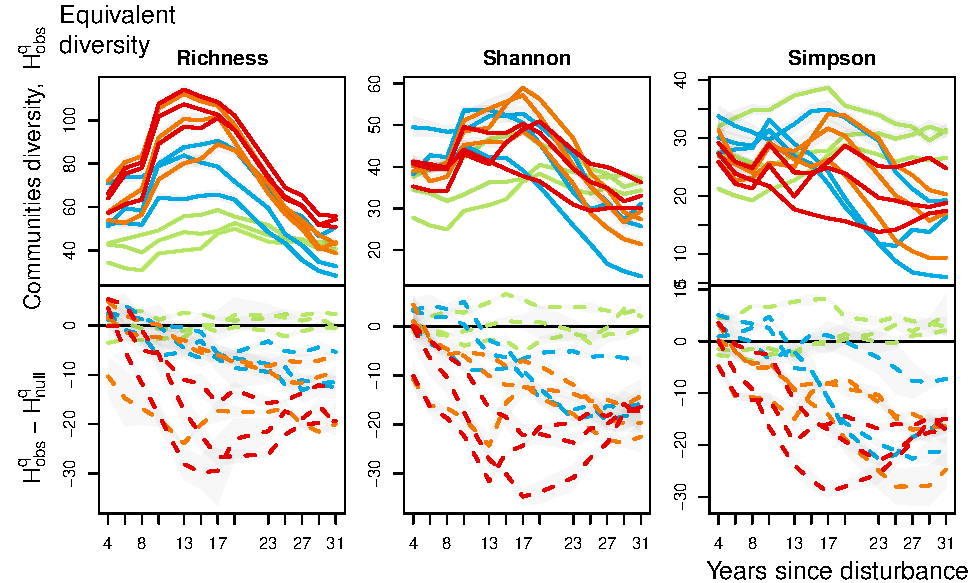
\includegraphics[width=0.8\linewidth]{RecruitmentTrajectories_files/figure-latex/Fig1-1} 

}

\caption{Trajectories of Richness, Shannon and Simpson diversity for 2-years laps punctual  recruitment (upper panels) and divergence to null model (lower panels). Lines colors refer to the perturbation regime: green for control, blue for T1, orange for T2 and red for T3 disturbance treatments. Plain lines correspond to the median observed after uncertainty propagation and are given along with the 95\% confidence interval (grey envelope).}\label{fig:Fig1}
\end{figure*}

\begin{figure*}

{\centering 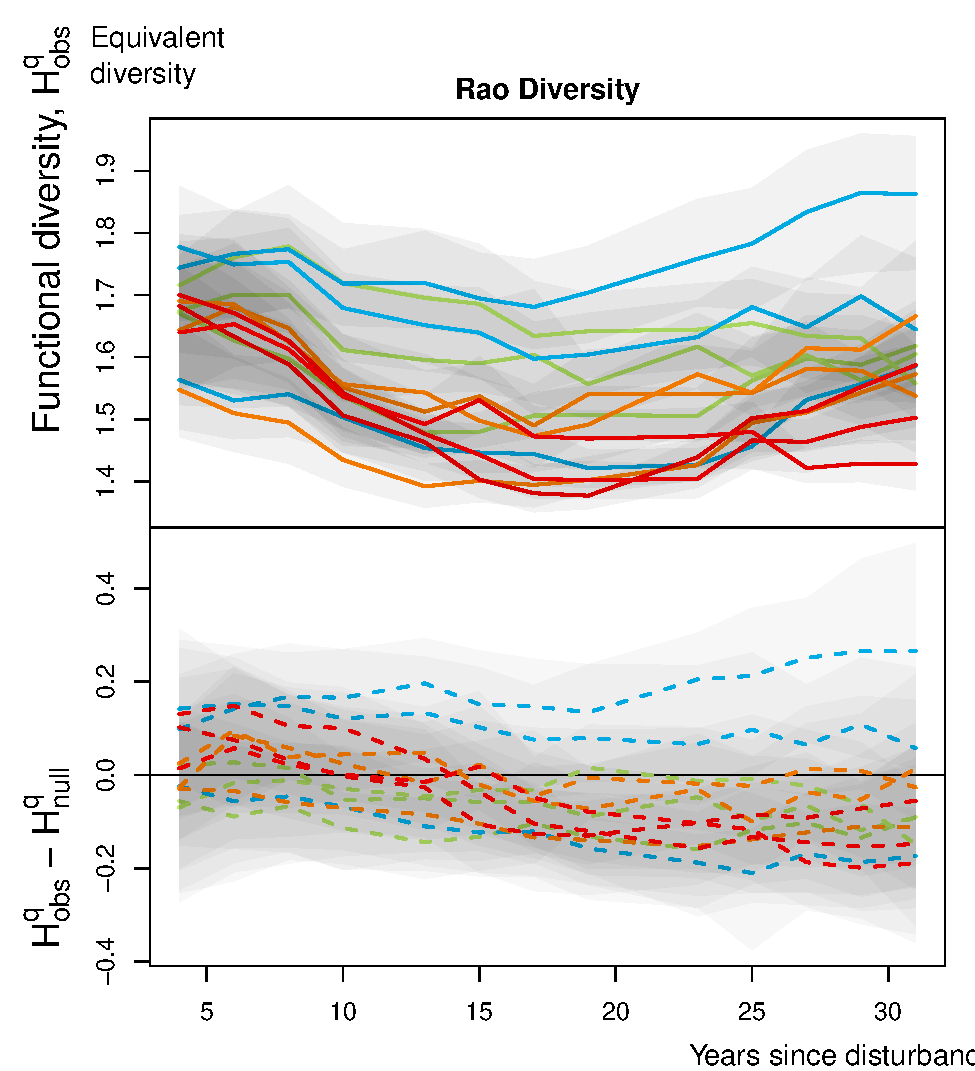
\includegraphics[width=0.8\linewidth]{RecruitmentTrajectories_files/figure-latex/Fig2-1} 

}

\caption{Trajectories of Richness, Shannon and Simpson diversity for 2-years laps accumulated recruitment (upper panels) and divergence to null model (lower panels). Lines colors refer to the perturbation regime: green for control, blue for T1, orange for T2 and red for T3 disturbance treatments. Plain lines correspond to the median observed after uncertainty propagation and are given along with the 95\% confidence interval (grey envelope).}\label{fig:Fig2}
\end{figure*}

Punctual and accumulated recruitment diversity of orders 0, 1 and 2 were
then compared to a null recruitment model with random sampling. In
control plots, punctual recruitment values were constantly equivalent or
higher than with the null model (Figure \ref{fig:Fig1}). In disturbed
plots, punctual recruitment richness (order 0) remained equivalent to
that of the null model but evenness (order 2) was first equivalent and,
after 10 years, became and remained lower than that of the null model.
Similar trajectories were observed for accumulated recruitments (Figure
\ref{fig:Fig2}).

-\textgreater{} Accumulated rajectories plots should go in SUPP MAT

\subsubsection{Functional diversity}\label{functional-diversity}

\begin{figure}

{\centering 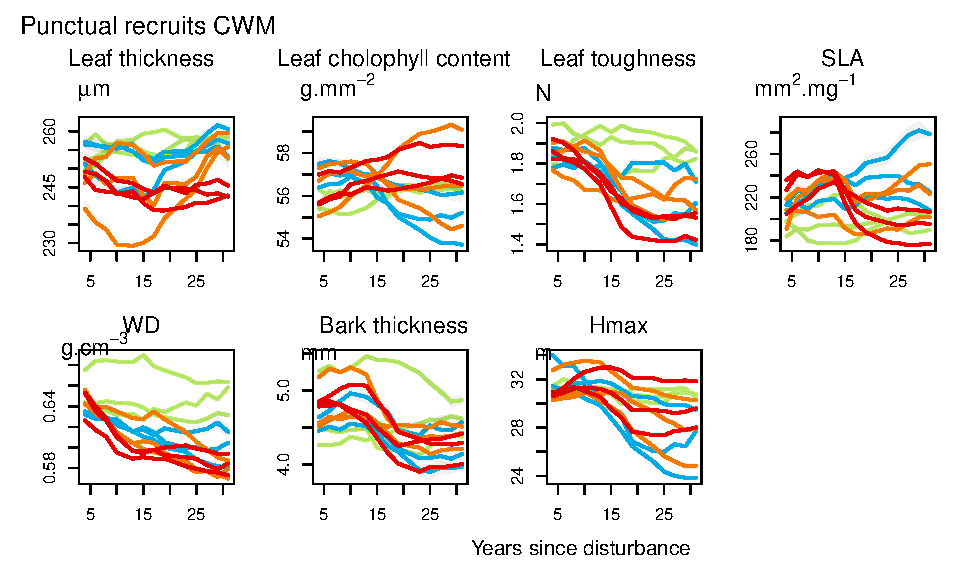
\includegraphics[width=0.8\linewidth]{RecruitmentTrajectories_files/figure-latex/Fig3-1} 

}

\caption{Functional diversity of punctual recruited trees from the considered functional traits and divergence to null model. Values reported correspond to the plot-level median and the 95\% confidence interval obtained after 50 repetition of the taxonomic uncertainty propagation and the functional database gap-filling processes and 50 run of the null model. Lines colors correspond to the logging treatment initially applied (green for control, blue for T1,orange for T2 and red for T3).}\label{fig:Fig3}
\end{figure}

Recruits functional diversity displayed a unimodal response to
disturbance with a maximum value positively linked to disturbance
intensity (R= xx) but with a time at maximum that was inversely related
to the disturbance treatment (R= xx) (Figure \ref{fig:Fig3}).
Trajectories of recruited trees in the functional spaces showed the
dominance after disturbance of species displaying large exchange surface
area and light tissues (high SLA, low leaf toughness and low wood
specific gravity) (Figure \ref{fig:Fig4}). All traits trajectories
displayed univariate CWM trajectories, except SLA and leaf thickness
that displayed a unimodal trajectory.

\begin{figure*}

{\centering 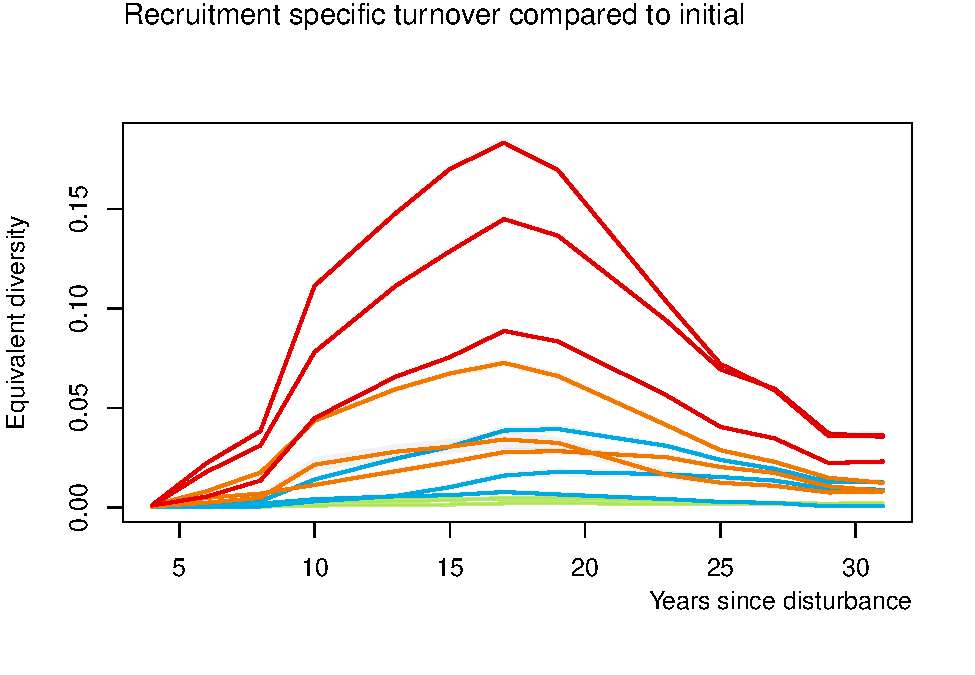
\includegraphics[width=0.8\linewidth]{RecruitmentTrajectories_files/figure-latex/Fig4-1} 

}

\caption{Community weighted means (CWM) of the four disturbance treatment for the four leaf traits, the two stem traits  and the specific Hmax. Values reported correspond to the plot-level median obtained after 50 repetition of the taxonomic uncertainty propagation and the functional database gap-filling processes. Lines colors correspond to the disturbance intensity (green for control, blue for T1,orange for T2 and red for T3).}\label{fig:Fig4}
\end{figure*}

\subsection{Recruitment Turnover}\label{recruitment-turnover}

In control plots, species turnover remained highly stable for the 30
sampled years (Figure \ref{fig:Fig5}). In disturbed plots, turnover
displayed a unimodal response to disturbance, with maximum reached
around 15 years and with a value positively correlated to the
disturbance intensity (R= xx). The turnover trajectory returned close to
zero for all plots 30 years after disturbance.

\begin{figure}

{\centering 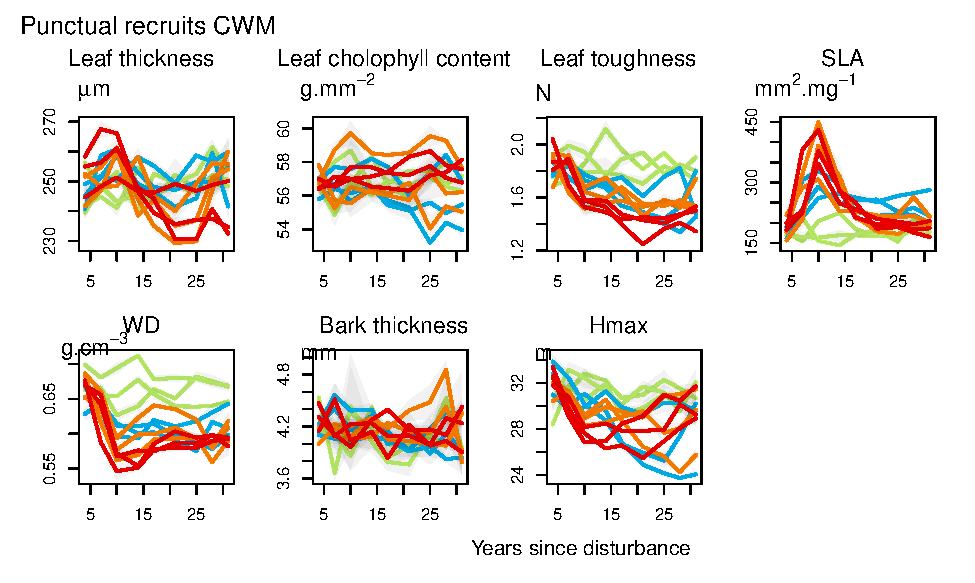
\includegraphics[width=0.5\linewidth]{RecruitmentTrajectories_files/figure-latex/Fig5-1} 

}

\caption{Trajectories over the 30 sampled years of the abundance-based turnover between recruited trees and intial communities before disturbance. Grey envelopes correspond to the 0.025 and 0.975 percentiles of the uncertainty propagation procedue and lines to the median in green for control, blue for T1,orange for T2 and red for T3).}\label{fig:Fig5}
\end{figure}

\section{Discussion}\label{discussion}

From the 30 years of forest dynamics survey in the Paracou station, we
highlighted contrasting recruitment patterns depending on disturbance
intensity. Disturbance increased the recruitment rate which subsequently
increased the richness of recruitment but impaired its evenness, all the
more so that disturbance intensity was high. After disturbance the
recruitment was dominated by a restricted pool of species and Shannon
and Simpson diversities decreased down to lower values than those of
control plots.

\subsection{On the underlyings of the hump-shaped
trajectories}\label{on-the-underlyings-of-the-hump-shaped-trajectories}

Punctual recruitment, some key functional traits (SLA, leaf thickness)
and turn-over trajectories exhibited hump-shaped curves so that, for the
10-15 first years following disturbance, recruitment processes seemed
first driven by the growth of pre-disturbance saplings that benefitted
from the environmental changes \citep{Herault2010} and progressively
incorporated true recruits, i.e.~individual trees that had germinated
after the disturbance. This translated by a regular increase in
functional diversity of recruits in the early times. According to the
SLA trajectory (Figure \ref{fig:Fig4}), these true recruits are mainly
pionneer species that dominate the recruited community 12 years after
disturbance.

After this first recruitment phase, in the case of low disturbance
intensity (T1 plots) the recruitment was higly similar to the
pre-disturbance community as revealed by the random sampling. This
argues for the existence of recruitment limitation in the medium-term
\emph{????meaning the strive of a variety of species, even when not the
most fitted for the environmental context, because the best competitors
couldn't set in disturbed area???? to be rewritten}. The key role of
recruitment limitation in recovery dynamic was already highlighted for
low disturbance intensity in tropical wet forests
\citep{Hubbell1999, Sheil2003, Bongers2009} and supported the IDH as it
mitigates competitive exclusion and maintains some inferior competitiors
in the community. Recruitment and dispersal limitation are consistent
with the short dispersal distance observed for tropical trees, and it
was already highlighted in Paracou through the genetic clumping observed
for some pioneers \citep{Leclerc2015, Scotti2015a}.

In the case of high disturbance intensity, the species turnover remains
very high after the initial 10 year phasis and the functional diversity
decreased sharply, along a general functional shift towards acquisitive
functional strategies. This was marked for nearly all functional traits
of the leaf and stem and for life history traits (Leaf thickness, Wood
Specific Gravity and Hmax) which values represented a community of
fast-growing long-lived species with a high resources acquisition
strategies \citep{Wright2004, Chave2009b, Herault2011, Reich2014}. The
time elpased between disturbance and the significance of those
functional and diversity shifts suggests that the second recruitment
phase stems from the germination of long-lived pioneers at the moment of
the disturbance. \emph{here i think that we are seeing the effect of
long-lived pioneers, and this should be discusssed. especially the
functional differences between long- and short-lived pioneers}

\emph{?????Eventually, we observed that disturbance induced particular
recruitment mechanisms but also set aside mechanisms at stake in natural
plots.????}

\subsection{On the resilience of the recruitment
process}\label{on-the-resilience-of-the-recruitment-process}

Thirty years after the disturbance event, the functional diversity
\emph{not true for all traits, i.e.~wood density} had recovered whatever
the disturbance intensity but significant taxonomic diversity difference
persisted for high disturbance levels. Would this mean that ecosystem
functioning recover faster than taxonomic composition? The link between
functional traits and ecpsystem functionning is not trivial but our
results may highlight the key role of functional redundancy in
ecological systems and also suggest that the recovery trajectory may be,
more than commonly thought, upon dependence of the pre-disturbance
functional ecosystem signature \citep{Herault2018}. Whatever the
disturbance intensity, the recruitment turnover compared to initial
stand ended up close to zero. This again argue for the high dependence
of the recovery trajectory on the pre-disturbance ecosystem
characteristics \citep{Anderson2007}. In other words, initial
compositional variation caused tree communities to remain divergent in
taxonomic composition, even though these same tree communities strongly
converged in functional space \citep{Fukami2005}. This makes these
commmunities both highly functionally and taxonomically resilient. Our
results extend previous ones from the Paracou experiment, 10 years
\citep{Molino2001} and 20 years \citep{Baraloto2012a} after disturbance
that suggested the recovery towards pre-disturbance taxonomic and
functional composition. This is however only valid for a single
disturbance event, given that second recruitment phase assumed to rely
on the seed bank triggers a storage effect likely to modify the
recruitment trajectories in case of a new disturbance event. In this
hypothetical case, the competitive exclusion among dormant life-stage
(seeds or even seedlings) would be harsher and would bring more radical
changes in the recruitment composition and functional profile.

\subsection{Conclusion}\label{conclusion}

Our long-term study of diversity trajectories after disturbance
disentangled the mechanisms underlying the forest trajectory in the
diversity space. While, in undisturbed forests, mechanisms like negative
density dependence enhanced species diversity, a single disturbance
event induced new mechanisms depending on the event intensity. Whatever
the intensity, communities short-term response reflected the enhanced
growth of already grown saplings which increased the taxonomic and
functional evenness of the community. In the long-term, the community
trajectory strongly depends on the disturbance intensity. For low
intensity, recruitment limitation was balanced against environmental
filters and induced a recruited community mirroring the pre-disturbance
community composition. For high intensity, the species turnover remains
very high and induced a recruited community significantly dominated by
acquisitive functional types and a restricted pool of species. \emph{In
both cases, the recruitment trajectory is specific, because it is
determined by the surrounding forest in case of low disturbance or
because the competitive exclusion randomly selected a restricted pool of
species after intense disturbance.?????}

\begin{center}\rule{0.5\linewidth}{\linethickness}\end{center}

%----------------------------------------------------------------------------------------
%	REFERENCE LIST
%----------------------------------------------------------------------------------------

\bibliographystyle{mee}
\bibliography{references.bib}

%----------------------------------------------------------------------------------------

\end{document}
